\section{Details on Real-Data Examples}
\subsection{ICU Mortality Example}
\label{appendix:icu_details}

This appendix provides full details on how we constructed the ICU data subsets, prepared the analytic dataset, estimated the OBD, identified sign reversals, and computed bootstrap standard errors for all data subsets used in \cref{sec:real_example}. The analyses use the PhysioNet ICU cohort collected for the study of in-hospital mortality \citep{goldberger2000physiobank}. The raw cohort contains routine admission measurements for $3,997$ patients with known gender ($2,246$ women and $1,751$ men). We merge these records with the corresponding mortality outcomes and restrict attention to patients with complete information on the covariates used in the decomposition: age, ICU type, heart rate (HR), mean arterial pressure (MAP), temperature, urine output, and the indicator for in-hospital death. After removing observations with missing covariates, the final analytic dataset contains $3,429$ patients. All data subset definitions, model specifications, and statistical procedures described below are applied to this cleaned dataset.

\subsection*{Model specification}

For each data subset, we fit separate group-specific models of in-hospital mortality for men and for women. Let $g \in \{\text{men}, \text{women}\}$, let $Y$ be the indicator for in-hospital mortality, and let $X$ be the vector of admission covariates (heart rate, mean arterial pressure, temperature, urine output, age, and ICU type). For each group $g$, we fit an estimator $\hat{M}_g(X)$ of the conditional expectation $\E[Y \mid X, g]$ and use \cref{eq:OB_H_Counterfactual,eq:OB_K_Counterfactual}; see \cref{sec:ob_real}. We consider five model classes, specified as follows.

\textbf{Linear regression.} We take
\[
    \E[Y \mid X, g] \;=\; \alpha_{g} + X^{\top}\beta_{g},
\]
with the group-specific intercept $\alpha_{g}$ and slope $\beta_{g}$ estimated by ordinary least squares. Although $Y$ is binary, this linear probability model is the object to which the classical OBD applies and remains standard in applied work \citep{jann2008, edokaChangesCatastrophicHealth2017, sujin_LPM_OB, mweembaGapSelfRatedHealth2023}.

\textbf{Logistic regression.} Within each group, we standardize the covariates to zero mean and unit variance and fit a logistic regression of $Y$ on the standardized covariates with the default $L_2$ penalty.

\textbf{Neural network.} Within each group, we standardize the covariates and fit a two-hidden-layer fully-connected ReLU network with hidden widths $(32, 16)$, $L_2$ weight decay $10^{-4}$, the Adam optimizer \citep{kingma2015adam}, and max\_iter $=2000$.

\textbf{XGBoost.} We fit a gradient-boosted tree classifier with $250$ estimators, maximum depth $3$, learning rate $0.05$, row subsampling rate $0.9$, column subsampling rate $0.9$, $L_2$ leaf regularization $\lambda = 1.0$, histogram tree method, and the logistic (log-loss) objective.

\textbf{TabPFN.} We use a modern transformer-based tabular model, TabPFN \citep{hollmann2023tabpfn}\footnote{TabPFN uses a custom license: \url{https://huggingface.co/Prior-Labs/tabpfn_2_6/blob/main/LICENSE}}, a pre-trained in-context classifier that maps a training set directly to a predictive distribution for $Y \mid X$. We use the publicly released v2.6 weights and use the v7.1.1 TabPFN code for inference. We run the model locally on a single NVIDIA A100 GPU with $80$~GB of vRAM.

For all five models, we take the predicted probability of in-hospital death as $\hat{M}_g(X)$ and estimate each NOBD counterfactual mean $\E_{g'}[\E_g[Y \mid X]]$ by the within-sample average $\frac{1}{|g'|}\sum_{i \in g'} \hat{M}_g(X_i)$.

\subsection*{Data subset construction}
The goal of this analysis was not to target any particular physiological pattern, but rather to explore systematically whether sign reversals arise in realistic data partitions that a practitioner might naturally encounter.

We constructed $139$ data subsets in total. These sets include: quartiles of each continuous admission vital (heart rate, MAP, temperature, urine output);
deciles of age; ICU-type specific cohorts; clinically motivated threshold subsets (HR $>100$, MAP $<65$, Temp $> 38^\circ$C, Urine $>1000$ mL); fifty random $50\%$ subsamples of the cohort; fifty random $30\%$ subsamples of the cohort.

For each data subset and each of the five models in our model class, we compute the decomposition under both reference groups, taking men and women in turn. We say that the explained or unexplained component sign flips in that data subset if its estimated value has opposite signs under the two reference choices. To assess whether such flips are robust to sampling variability, we next describe the bootstrap procedure we use to compute standard errors and $p$-values for each component.

\textbf{Bootstrap.}
For each data subset and each model, we compute bootstrap standard errors and $p$-values for the OBD components. The bootstrap procedure follows the standard Oaxaca--Blinder framework: men and women are resampled within group with replacement, preserving group sizes. For each bootstrap replication $b=1,\dots,B$, we re-fit the corresponding group-specific model and re-estimate the OBD components.

Let $\hat\theta$ denote any Oaxaca--Blinder component (for example, the explained component under the women reference model), and let $\hat\theta^{(1)},\dots,\hat\theta^{(B)}$ denote its bootstrap replicates. The bootstrap standard error and mean are
\[
    \widehat{\operatorname{se}}(\hat\theta)
    =
    \sqrt{
    \frac{1}{B-1}\sum_{b=1}^B
    \bigl(\hat\theta^{(b)} - \bar\theta\bigr)^2
    },
    \qquad
    \bar\theta = \frac{1}{B}\sum_{b=1}^B \hat\theta^{(b)}.
\]
$P$-values are computed using a normal approximation,
\[
    p = 2\left(1 - \Phi\left(\frac{|\hat\theta|}{\widehat{\operatorname{se}}(\hat\theta)}\right)\right).
\]

We say that a sign flip is significant at level $\alpha$ if, in addition to having opposite signs across reference groups, at least one of the two reference-specific estimates has $p < \alpha$. We summarize the total number of data subsets exhibiting any sign flip under each model in \cref{tab:flip_summary_main} in \cref{sec:real_example}. Here, \cref{tab:flip_summary_explained,tab:flip_summary_unexplained} below report the same counts separately for the explained and unexplained components.

We observed that empirically, the count of data subsets exhibiting a sign flip grows with model complexity for this particular data analysis. With the linear and logistic models showing the least amount of sign flips and only a couple remain significant at conventional thresholds. While the neural network and XGBoost show a substantial fraction of data subsets exhibits significant flips even at the $5\%$ level. Importantly, many of the flipped data subsets arise within the random subsamples, indicating that the OBD can yield unstable conclusions even when applied to simple resampled partitions of the same population. Several physiologically interpretable groups also displayed sign changes. The HR quartile two data subset examined in \cref{sec:real_example} is one such case, and serves as a concrete illustration of how these reversals can appear in clinically meaningful settings.

\begin{table}[!ht]
    \caption{Number of data subsets (out of $139$) exhibiting a sign flip in the explained component, by model. Columns $10\%$, $5\%$, and $1\%$ report the number of flipped data subsets that are significant at the corresponding level.}
    \label{tab:flip_summary_explained}
    \centering
    \small
    \begin{tabular}{lcccc}
    \toprule
    Model & Total flips & $10\%$ & $5\%$ & $1\%$ \\
    \midrule
    Linear      & 11 &  2 &  2 &  2 \\
    Logistic    &  9 &  2 &  2 &  1 \\
    Neural net  & 42 & 26 & 17 &  6 \\
    XGBoost     & 33 & 17 & 10 & 3 \\
    TabPFN      & 33 & 21 & 19 & 5 \\
    \bottomrule
    \end{tabular}
\end{table}

\begin{table}[!ht]
    \caption{Number of data subsets (out of $139$) exhibiting a sign flip in the unexplained component, by model. Columns $10\%$, $5\%$, and $1\%$ report the number of flipped data subsets that are significant at the corresponding level.}
    \label{tab:flip_summary_unexplained}
    \centering
    \small
    \begin{tabular}{lcccc}
    \toprule
    Model & Total flips & $10\%$ & $5\%$ & $1\%$ \\
    \midrule
    Linear      & 17 &  0 &  0 &  0 \\
    Logistic    & 21 &  0 &  0 &  0 \\
    Neural net  & 49 & 10 &  6 &  1 \\
    XGBoost     & 47 & 3 &  1 &  0 \\
    TabPFN      & 56 & 2 &  0 &  0 \\
    \bottomrule
    \end{tabular}
\end{table}

A substantial number of these sign reversals are significant at conventional thresholds, indicating that the instability documented in \cref{sec:real_example} is an inherent behavior of the OBD in this clinical dataset.


% \begin{table}[!t]
%     \centering
%     \caption{ICU Mortality Gap Decomposition for Data Subsets Exhibiting Sign Reversals. Standard errors in parentheses computed via bootstrap resampling with $1{,}000$ replications.  
%     P-values based on a normal approximation.  
%     Significance levels: * $p<0.10$, ** $p<0.05$, *** $p<0.01$.  
%     The decomposition separates the gender mortality gap (male minus female) into explained and unexplained components using the Oaxaca--Blinder method.  
%     Female Reference uses the model for females as the reference outcome structure; Male Reference uses the model for males.}
%     \label{tab:icu_mortality}
%     \scriptsize
%     \begin{tabular}{@{}lc*{5}{c}@{}}
%     \toprule
%     \multirow{2}{*}{Subset} &
%     \multirow{2}{*}{n} &
%     Gap &
%     \multicolumn{2}{c}{Female Reference} &
%     \multicolumn{2}{c}{Male Reference} \\
%     \cmidrule(lr){3-3} \cmidrule(lr){4-5} \cmidrule(lr){6-7}
%     & & (M–F) & Expl. & Unexp. & Expl. & Unexp. \\
%     \midrule
    
%     Age decile 1 & 344 & 0.027 & 0.002 & 0.025 & 0.036$^{*}$ & $-0.009$ \\
%     & & (0.033) & (0.009) & (0.033) & (0.019) & (0.030) \\[0.3em]
    
%     Age decile 2 & 347 & 0.004 & 0.023 & $-0.019$ & $-0.010$ & 0.015 \\
%     & & (0.033) & (0.021) & (0.041) & (0.014) & (0.036) \\[0.3em]
    
%     Age decile 4 & 372 & $-0.015$ & 0.012 & $-0.027$ & $-0.004$ & $-0.012$ \\
%     & & (0.032) & (0.013) & (0.035) & (0.017) & (0.037) \\[0.3em]
    
%     Age decile 5 & 344 & $-0.025$ & 0.010 & $-0.035$ & $-0.008$ & $-0.017$ \\
%     & & (0.039) & (0.016) & (0.039) & (0.022) & (0.042) \\[0.3em]
    
%     Age decile 9 & 325 & $-0.077$ & 0.001 & $-0.078$ & 0.001 & $-0.078$ \\
%     & & (0.048) & (0.023) & (0.049) & (0.013) & (0.049) \\[0.3em]
    
%     \textbf{HR quartile 2} & 816 & 0.035 & 0.021$^{***}$ & 0.014 & $-0.007$ & 0.042$^{*}$ \\
%     & & (0.023) & (0.007) & (0.025) & (0.011) & (0.025) \\[0.3em]
    
%     MAP quartile 0 & 877 & $-0.014$ & $-0.003$ & $-0.011$ & 0.004 & $-0.018$ \\
%     & & (0.026) & (0.009) & (0.026) & (0.008) & (0.026) \\[0.3em]
    
%     MAP quartile 1 & 840 & 0.024 & 0.036$^{***}$ & $-0.012$ & 0.011 & 0.013 \\
%     & & (0.022) & (0.012) & (0.027) & (0.008) & (0.022) \\[0.3em]
    
%     Urine quartile 0 & 859 & $-0.031$ & 0.007 & $-0.038$ & $-0.006$ & $-0.025$ \\
%     & & (0.027) & (0.009) & (0.027) & (0.007) & (0.027) \\[0.3em]
    
%     MAP $< 65$ & 697 & $-0.028$ & $-0.011$ & $-0.017$ & 0.002 & $-0.030$ \\
%     & & (0.029) & (0.012) & (0.029) & (0.008) & (0.029) \\[0.3em]
    
%     Temp $> 36.5$ & 267 & $-0.043$ & $-0.001$ & $-0.042$ & 0.008 & $-0.051$ \\
%     & & (0.047) & (0.025) & (0.050) & (0.019) & (0.046) \\[0.3em]
    
%     Urine $> 1000$ & 210 & 0.046 & $-0.014$ & 0.060 & 0.014 & 0.031 \\
%     & & (0.036) & (0.018) & (0.038) & (0.023) & (0.037) \\[0.3em]
    
%     Random 50\% \#6 & 1714 & 0.020 & 0.023$^{***}$ & $-0.003$ & 0.012$^{**}$ & 0.009 \\
%     & & (0.017) & (0.005) & (0.018) & (0.006) & (0.017) \\[0.3em]

%     Random 50\% \#21 & 1714 & 0.018 & 0.019$^{***}$ & $-0.001$ & 0.015$^{***}$ & 0.003 \\
%     & & (0.016) & (0.005) & (0.017) & (0.005) & (0.015) \\[0.3em]

%     Random 50\% \#28 & 1714 & 0.013 & 0.016$^{***}$ & $-0.004$ & 0.009$^{**}$ & 0.003 \\
%     & & (0.018) & (0.005) & (0.018) & (0.004) & (0.017) \\[0.3em]

%     Random 50\% \#30 & 1714 & 0.008 & 0.014$^{***}$ & $-0.006$ & 0.004 & 0.005 \\
%     & & (0.017) & (0.005) & (0.018) & (0.004) & (0.017) \\[0.3em]

%     Random 50\% \#34 & 1714 & 0.009 & 0.016$^{***}$ & $-0.007$ & 0.009$^{*}$ & 0.001 \\
%     & & (0.015) & (0.005) & (0.016) & (0.005) & (0.015) \\[0.3em]

%     Random 50\% \#39 & 1714 & 0.019 & 0.020$^{***}$ & $-0.001$ & 0.012$^{**}$ & 0.007 \\
%     & & (0.017) & (0.005) & (0.018) & (0.005) & (0.016) \\[0.3em]

%     Random 30\% \#0 & 1028 & 0.018 & 0.018$^{***}$ & $-0.001$ & 0.008 & 0.010 \\
%     & & (0.022) & (0.006) & (0.023) & (0.006) & (0.021) \\[0.3em]

%     Random 30\% \#5 & 1028 & 0.011 & 0.016$^{***}$ & $-0.005$ & 0.008 & 0.003 \\
%     & & (0.020) & (0.006) & (0.021) & (0.008) & (0.021) \\[0.3em]

%     Random 30\% \#17 & 1028 & 0.008 & 0.014$^{**}$ & $-0.006$ & 0.008 & 0.000 \\
%     & & (0.022) & (0.007) & (0.023) & (0.006) & (0.022) \\[0.3em]

%     Random 30\% \#18 & 1028 & 0.007 & 0.022$^{***}$ & $-0.015$ & 0.002 & 0.004 \\
%     & & (0.022) & (0.007) & (0.024) & (0.005) & (0.022) \\[0.3em]

%     Random 30\% \#20 & 1028 & 0.002 & 0.001 & 0.001 & 0.005 & $-0.003$ \\
%     & & (0.020) & (0.007) & (0.020) & (0.005) & (0.019) \\[0.3em]

%     Random 30\% \#24 & 1028 & 0.021 & 0.018$^{***}$ & 0.003 & $-0.007$ & 0.027 \\
%     & & (0.021) & (0.007) & (0.023) & (0.010) & (0.023) \\[0.3em]

%     Random 30\% \#31 & 1028 & 0.015 & 0.014$^{**}$ & 0.000 & 0.023$^{***}$ & $-0.009$ \\
%     & & (0.021) & (0.007) & (0.022) & (0.009) & (0.020) \\[0.3em]

%     Random 30\% \#37 & 1028 & 0.011 & 0.021$^{**}$ & $-0.011$ & 0.007 & 0.004 \\
%     & & (0.023) & (0.009) & (0.025) & (0.006) & (0.022) \\[0.3em]

%     Random 30\% \#43 & 1028 & 0.015 & 0.017$^{**}$ & $-0.002$ & 0.012$^{**}$ & 0.003 \\
%     & & (0.021) & (0.007) & (0.023) & (0.006) & (0.021) \\
    
%     \bottomrule
%     \end{tabular}
% \end{table}
    
\subsection*{HR quartile 2: results across models}
\label{appendix:hrq2}

\cref{sec:real_example} focuses on the HR quartile two data subset under the OBD. In \cref{tab:hrq2_bootstrap_models}, we report the corresponding decomposition under each of the five models in our model class. The linear, logistic, neural-network, and XGBoost results are obtained from the bootstrap procedure described above with $B = 1{,}000$ replications.

% table* because the appendix is set in two columns (layout only).
\begin{table*}[!ht]
    \caption{OBD of the gender mortality gap in HR quartile two ($n = 816$), across all five models. The total gap is men's mean minus women's mean. Standard errors in parentheses are computed via bootstrap resampling with $1{,}000$ replications. $p$-values are based on a normal approximation (Wald test). Significance levels: * $p<0.10$, ** $p<0.05$, *** $p<0.01$.}
    \label{tab:hrq2_bootstrap_models}
    \centering
    \scriptsize
    \begin{tabular}{@{}lc*{4}{c}@{}}
    \toprule
    \multirow{2}{*}{Model} &
    \multirow{2}{*}{Gap (M--F)} &
    \multicolumn{2}{c}{Women reference} &
    \multicolumn{2}{c}{Men reference} \\
    \cmidrule(lr){3-4} \cmidrule(lr){5-6}
    & & Explained & Unexplained & Explained & Unexplained \\
    \midrule

    Linear
        & \makecell{$0.035$ \\ $(0.023)$}
        & \makecell{$0.021^{***}$ \\ $(0.007)$}
        & \makecell{$0.014$ \\ $(0.025)$}
        & \makecell{$-0.007$ \\ $(0.010)$}
        & \makecell{$0.042^{*}$ \\ $(0.025)$} \\[0.3em]

    Logistic
        & \makecell{$0.035$ \\ $(0.023)$}
        & \makecell{$0.026^{***}$ \\ $(0.009)$}
        & \makecell{$0.009$ \\ $(0.025)$}
        & \makecell{$-0.006$ \\ $(0.008)$}
        & \makecell{$0.041^{*}$ \\ $(0.024)$} \\[0.3em]

    Neural net
        & \makecell{$0.035$ \\ $(0.023)$}
        & \makecell{$0.001$ \\ $(0.024)$}
        & \makecell{$0.033$ \\ $(0.031)$}
        & \makecell{$0.053^{**}$ \\ $(0.022)$}
        & \makecell{$-0.018$ \\ $(0.025)$} \\[0.3em]

    XGBoost
        & \makecell{$0.035$ \\ $(0.023)$}
        & \makecell{$0.004$ \\ $(0.016)$}
        & \makecell{$0.031$ \\ $(0.025)$}
        & \makecell{$0.029^{**}$ \\ $(0.014)$}
        & \makecell{$0.006$ \\ $(0.021)$} \\[0.3em]

    TabPFN
        & \makecell{$0.035$ \\ $(0.023)$}
        & \makecell{$0.012$ \\ $(0.016$}                                                                                                                                                                                                                                                                              
        & \makecell{$0.023$ \\ $(0.026)$}
        & \makecell{$0.023^{*}$ \\ $(0.013)$} 
        & \makecell{$0.012$ \\ $(0.021)$} \\[0.3em]
    \bottomrule
    \end{tabular}
\end{table*}

The linear and logistic OBD exhibit a consistent explained-component sign flip that is significant at the $1\%$ level, with very similar magnitudes: in both cases, the explained component is significantly positive under the women reference and flips to a small negative (non-significant) value under the men reference. The neural network and XGBoost both point to the men reference estimate being significantly positive at the $5\%$ level.

\cref{fig:hr_quartile2_hist} presents the histogram for the $816$ patients in HR quartile two, showing the distribution of mortality outcomes used in the linear probability models displayed in \cref{fig:sign_flip_overview} (left). \cref{tab:delta_mu_betas} shows the covariate mean differences and group-specific coefficients for HR quartile two that underlie the sign reversal documented in \cref{sec:real_example}.

\begin{figure}[!ht]
    %REV width=0.5\linewidth (two-column layout: now full column width)
    \centerline{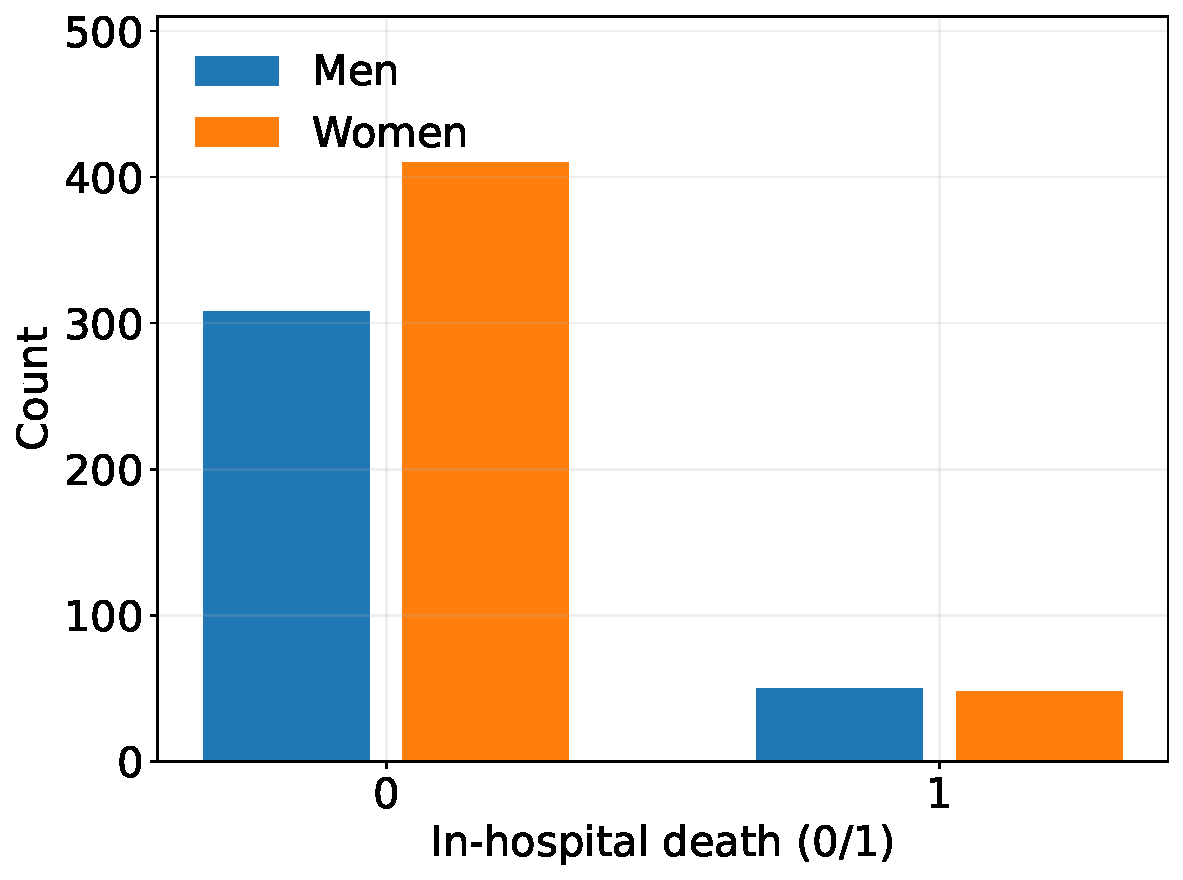
\includegraphics[width=\linewidth]{Sections/Figures/hr_quartile2_mortality_y_hist.pdf}}
    \caption{Mortality outcome histogram for HR quartile two data subset.}
    \label{fig:hr_quartile2_hist}
\end{figure}

\begin{table}[!ht]
    \caption{Covariate mean differences and group-specific coefficients in HR quartile two. $\Delta\mu$ denotes the difference in covariate means between men and women within HR quartile two (men minus women). $\beta_{\text{Men}}$ and $\beta_{\text{Women}}$ are coefficients from group-specific linear probability models for in-hospital mortality.}
    \label{tab:delta_mu_betas}
    \centering
    \small
    \begin{tabular}{lrrr}
    \toprule
    Covariate 
    & $\Delta\mu$ 
    & $\beta_{\text{Men}}$ 
    & $\beta_{\text{Women}}$ \\
    \midrule
    Intercept & $0.0000$   & $1.1813$  & $-0.8515$ \\
    Age       & $3.8938$   & $-0.0000$ & $0.0039$ \\
    ICU Type  & $0.0095$   & $0.0173$  & $0.0116$ \\
    HR        & $0.4982$   & $-0.0026$ & $0.0056$ \\
    MAP       & $-0.6669$  & $0.0004$  & $0.0010$ \\
    Temp      & $0.3604$   & $-0.0230$ & $0.0028$ \\
    Urine     & $-39.8976$ & $-0.0001$ & $-0.0001$ \\
    \bottomrule
    \end{tabular}
\end{table}
    
\subsection{U.S.\ Labor Force Example}
\label{appendix:us_labor_force}
This appendix provides full details on how we constructed the U.S.\ labor force \textcolor{red}{data subsets}, prepared the analytic dataset, estimated the (N)OBD, and identified sign reversals for all \textcolor{red}{data subsets}. %REV subgroups ... subgroups
 
The raw data come from the 2016 American Community Survey 1-Year Public Use Microdata Sample, which contains 1,625,282 observations.
We apply the same sample construction as \citet{bach2024heterogeneity}, who study the gender wage gap.
We restrict the sample to adults between the ages of 25 and 65, who were employed and at work as civilians, worked at least 35 hours per week, at least 50 weeks per year, and with both earnings and income above \$12,687.50 (which corresponds conservatively to an hourly wage of \$7.25).
The resulting sample contains 871,849 observations.

We purposely construct a large set of analyses to search for sign flips in different subsets of the data, comprising all combinations of the factors in \cref{tab:us_census_design}.

\begin{table}[!ht]
    \caption{Settings for sign flip search in the U.S.\ labor force dataset.}
    \label{tab:us_census_design}
    \centering
    \footnotesize
    \setlength{\tabcolsep}{4pt}
    \begin{tabular}{@{}ll@{}}
    \toprule
    Subset \( S \) & Group (\( H, K \)) \\
    \midrule
    26 industries (NAICS 2) & Race (black, white)                  \\
    50 states + D.C,        & Sex (male, female)                   \\
                            & Nativity (native born, foreign born) \\
    \bottomrule
    \end{tabular}
\end{table}

There are \( 77 \times 3 = 231 \) combinations of subsets and groups, each corresponding to a particular \textcolor{red}{data subset} an analyst could perform the (N)OBD within. %REV subgroup

We consider two outcomes: the natural logarithm of income (the outcome from \citet{bach2024heterogeneity}), and a binary indicator for having health insurance.
We exclude 11 cases where there are fewer than 50 observations in either $H$ or $K$ (), or $|\Delta Y| < 50$; this intended to focus more on analyses where the data may be informative and differences in outcomes may be practically meaningful.
The result is 217 \textcolor{red}{data subsets} for log-income, and 183 \textcolor{red}{data subsets} for health insurance status. %REV subgroups ... subgroups

For each analysis, we assemble a candidate feature set from state of residence, industry of occupation (NAICS 2 code), sex, race (black, white, or other), nativity, completion of a Bachelor's degree, and marital status.
We exclude features that define the particular subset and group at hand, to produce a feature set for model fitting.
For example, when examining male-female differences in the state of Wyoming, we remove sex and state from the feature set.

We then perform the (N)OBD by estimating $\E[Y \mid X, g, s]$ with the specified model, 
where \( Y \) and \( X \) are the outcome and covariates, 
\( g \) indexes the group (i.e. male or female sex);
and \( s \) indicates a subset of the data (i.e., the state of Utah).
The models are:
\begin{itemize}
    \item Ordinary least squares regression.
    \item Logistic regression (when $Y$ is binary), \textcolor{red}{with the default $L_2$ penalty as in \cref{appendix:icu_details}}. %REV unpenalized.
    \item \textcolor{red}{XGBoost, the neural network, and TabPFN, with the specifications of \cref{appendix:icu_details}; for the continuous log-income outcome, we use the corresponding regressors with the same hyperparameters.}
%REV     \item lightgbm (gradient-boosted trees). We set a learning rate of 0.25, number of leaves to 7, and select the number of trees by 3-fold cross-validation with early stopping at 10 rounds. All other parameters are set to default values.
\end{itemize}
%REV We attempted to implement neural networks for regression (both outcomes) and classification (health insurance status only), but faced repeated software errors while optimizing model weights.
We use the same bootstrap inference procedure as in \cref{appendix:icu_details}\textcolor{red}{, with $1{,}000$ replications}. %REV for ordinary least squares and logistic regression. 
%REV We do not perform inference for lightgbm due to computational costs of bootstrapping; future work can assess the statistical significance of the results with appropriate resources.
All computation was performed on an Apple M2 Max chip with 32GB ram.

\cref{tab:flips_census_income,tab:flips_census_insurance} report the number of sign flips for the log income and health insurance status outcomes, respectively.
Sign flips occur in both the explained and unexplained components for all tested model types.

% Log income. table* because the appendix is set in two columns. Values: census/out_py/flip_counts.csv (Python pipeline, B = 1000).
\begin{table*}[!ht]
    \caption{Number of \rc{data subsets} (out of $217$) exhibiting a sign flip in the explained and unexplained component, for the earnings outcome. Columns $10\%$, $5\%$, and $1\%$ report the number of flipped data subsets that are significant at the corresponding level.} %REV No significance testing was performed for lightgbm due to computational costs of bootstrap inference.
    \label{tab:flips_census_income}
    \centering
    \small
    \begin{tabular}{l*{12}{c}}
    \toprule
          & \multicolumn{4}{c}{Either Component} & \multicolumn{4}{c}{Explained Component} & \multicolumn{4}{c}{\rc{Unexplained} Component} \\
          \cmidrule(lr){2-5} \cmidrule(lr){6-9} \cmidrule(lr){10-13}
    Model       & Total & $10\%$ & $5\%$ & $1\%$ & Total & $10\%$ & $5\%$ & $1\%$ & Total & $10\%$ & $5\%$ & $1\%$ \\
    \midrule
    Linear      & \rc{33} & \rc{16} & \rc{13} & \rc{8} & \rc{21} & \rc{11} & \rc{9} & \rc{6} & \rc{13} & \rc{5} & \rc{4} & \rc{2} \\
    \rc{Neural net} & \rc{87} & \rc{--} & \rc{--} & \rc{--} & \rc{83} & \rc{--} & \rc{--} & \rc{--} & \rc{12} & \rc{--} & \rc{--} & \rc{--} \\
    \rc{XGBoost}    & \rc{34} & \rc{18} & \rc{16} & \rc{12} & \rc{31} & \rc{15} & \rc{14} & \rc{11} & \rc{5} & \rc{4} & \rc{3} & \rc{2} \\
    \rc{TabPFN}     & \rc{--} & \rc{--} & \rc{--} & \rc{--} & \rc{--} & \rc{--} & \rc{--} & \rc{--} & \rc{--} & \rc{--} & \rc{--} & \rc{--} \\
%REV Linear      & 35 & 14 & 11 & 7 & 24 & 10 & 8 & 5 & 11 & 4 & 3 & 2 \\
%REV lightgbm    & 29 & -  & -  & - & 23 & -  & - & - & 6  & - & - & - \\
    \bottomrule
    \end{tabular}
\end{table*}

% Health insurance. table* because the appendix is set in two columns. Values: census/out_py/flip_counts.csv (Python pipeline, B = 1000; logistic = L2, the ICU specification).
\begin{table*}[!ht]
    \caption{Number of \rc{data subsets} (out of $183$) exhibiting a sign flip in the explained and unexplained component, for the (binary) health insurance status outcome. Columns $10\%$, $5\%$, and $1\%$ report the number of flipped data subsets that are significant at the corresponding level.} %REV No significance testing was performed for lightgbm due to computational costs of bootstrap inference.
    \label{tab:flips_census_insurance}
    \centering
    \small
    \begin{tabular}{l*{12}{c}}
    \toprule
          & \multicolumn{4}{c}{Either Component} & \multicolumn{4}{c}{Explained Component} & \multicolumn{4}{c}{\rc{Unexplained} Component} \\
          \cmidrule(lr){2-5} \cmidrule(lr){6-9} \cmidrule(lr){10-13}
    Model       & Total & $10\%$ & $5\%$ & $1\%$ & Total & $10\%$ & $5\%$ & $1\%$ & Total & $10\%$ & $5\%$ & $1\%$ \\
    \midrule
    Linear      & \rc{65} & \rc{38} & \rc{32} & \rc{23} & \rc{52} & \rc{37} & \rc{31} & \rc{23} & \rc{15} & \rc{2} & \rc{1} & \rc{0} \\
    Logistic    & \rc{62} & \rc{31} & \rc{25} & \rc{14} & \rc{45} & \rc{28} & \rc{23} & \rc{14} & \rc{18} & \rc{3} & \rc{2} & \rc{0} \\
    \rc{Neural net} & \rc{65} & \rc{--} & \rc{--} & \rc{--} & \rc{51} & \rc{--} & \rc{--} & \rc{--} & \rc{21} & \rc{--} & \rc{--} & \rc{--} \\
    \rc{XGBoost}    & \rc{54} & \rc{34} & \rc{26} & \rc{16} & \rc{45} & \rc{33} & \rc{25} & \rc{16} & \rc{10} & \rc{1} & \rc{1} & \rc{0} \\
    \rc{TabPFN}     & \rc{--} & \rc{--} & \rc{--} & \rc{--} & \rc{--} & \rc{--} & \rc{--} & \rc{--} & \rc{--} & \rc{--} & \rc{--} & \rc{--} \\
%REV Linear      & 60 & 35 & 33 & 24 & 44 & 33 & 31 & 23 & 17 & 2 & 2 & 1 \\
%REV Logistic    & 77 & 23 & 16 & 10 & 60 & 23 & 16 & 10 & 25 & 1 & 0 & 0 \\
%REV lightgbm    & 97 & -  & -  & -  & 23 & -  & - & - & 6  & - & - & - \\
    \bottomrule
    \end{tabular}
\end{table*}


\subsection{Sign Flips as a Function of Model Complexity}
\label{appendix:complexity}
{\color{red}
\cref{tab:flip_summary_main} shows more sign flips for the more flexible models on the ICU data. A natural question a practitioner might ask is whether these sign flips are an artifact of model selection or of the hyperparameter choices of the machine learning models, and what happens as we increase the complexity of a given model. %REV Our empirical results above show more sign flips for the more flexible models. A natural question is what happens as we increase the complexity of a given model.
 To answer it, we take the XGBoost and neural network models of \cref{appendix:icu_details} and vary one hyperparameter at a time, holding every other setting at the value given in \cref{appendix:icu_details}. We use exactly the $139$ ICU data subsets of \cref{tab:flip_summary_main} and the $217$ log-income and $183$ health-insurance data subsets of \cref{tab:flips_census_income,tab:flips_census_insurance}. For each setting, we count the subsets in which the explained component, the unexplained component, or either component has opposite signs under the two reference groups. We count sign flips of the point estimates and do not perform bootstrap inference, so these counts correspond to the ``Total'' columns of \cref{tab:flip_summary_main,tab:flips_census_income,tab:flips_census_insurance}. Linear and logistic regression have no comparable complexity knob and are not varied.

\textbf{XGBoost.} We vary the maximum tree depth over $\{1, \dots, 10\}$ with $250$ trees, and the number of trees over $\{10, 25, 50, 100, 250, 500, 1{,}000, 2{,}000, 4{,}000, 10{,}000\}$ with depth $3$. All other settings (learning rate $0.05$, row and column subsampling rates $0.9$, $\lambda = 1$, histogram tree method) are as in \cref{appendix:icu_details}; depth $3$ with $250$ trees is the model reported in \cref{tab:flip_summary_main,tab:flips_census_income,tab:flips_census_insurance}.

\textbf{Neural network.} We vary the width $w$ of a network with three hidden layers of equal width, $(w, w, w)$, over $w \in \{8, 16, 32, 64, 128, 256, 512, 768\}$ for the ICU data (up to $1.2 \times 10^6$ trainable parameters) and $w \in \{8, \dots, 256\}$ for the Census data (up to $1.5 \times 10^5$ parameters), where the largest widths are prohibitively slow on data subsets of up to $120{,}000$ workers. Separately, we vary the depth $d$ of a network with hidden layers of width $32$, $(32,) \times d$, over $d \in \{1, 2, 3, 4, 6, 8, 12, 16\}$. Each network in a sweep strictly contains the previous one, so complexity is increasing along each sweep. The ReLU activation, $L_2$ weight decay $10^{-4}$, Adam optimizer, maximum of $2{,}000$ iterations, and standardized inputs are as in \cref{appendix:icu_details}. Because the fitted network depends on its random initialization, we repeat every setting with three initialization seeds and report the mean and the range across seeds. The two-hidden-layer $(32, 16)$ network reported in \cref{tab:flip_summary_main,tab:flips_census_income,tab:flips_census_insurance} is not on either sweep; we mark its flip count with a dashed line.

\cref{fig:complexity_sweeps} reports the results. At the settings of \cref{tab:flip_summary_main,tab:flips_census_income,tab:flips_census_insurance}, every sweep reproduces the corresponding table entry (for XGBoost, $62$ subsets for the ICU data, $34$ for log income, and $54$ for health insurance).

\textbf{ICU data.} Every knob increases the number of sign flips. For XGBoost, the number of subsets with a flip in either component grows from $26$ at depth $1$ to $138$ of $139$ at depth $10$, and from $27$ with $10$ trees to $137$ with $10{,}000$ trees. For the neural network, it grows from $46$ to $97$ as the width increases to $128$ and then levels off between $85$ and $95$ at the largest widths; with depth, it grows from $33$ with one hidden layer to $76$ with four and then stays between $65$ and $71$.

\textbf{Census data.} The number of sign flips is nearly insensitive to complexity. For log income, XGBoost flips between $24$ and $40$ of $217$ data subsets across both sweeps, with a slight decrease at the most complex settings; wider networks flip between $67$ and $97$ data subsets, and deeper networks flip \emph{fewer} data subsets, from $96$ with one hidden layer to $43$ with sixteen. For health insurance, XGBoost flips between $47$ and $65$ of $183$ data subsets (except for very few trees, where it flips $21$--$34$), wider networks flip between $59$ and $73$, and deeper networks stay between $51$ and $62$.

We draw two conclusions. First, we do not observe a single relationship between model complexity and sign flips: the ICU data show a clear increase, while the Census data show none. Second, in neither dataset does increasing complexity remove sign flips; at every setting we consider, a substantial number of subsets flip sign. We leave the source of the difference between the two datasets to future work. We note that the Census data subsets are one to two orders of magnitude larger than the ICU subsets and that their covariates are predominantly indicators (state and industry), both of which may limit how differently two group-specific models can extrapolate to each other's covariate distribution.
}

\begin{figure*}[p]
    \centering
    {\color{red}
    \setlength{\tabcolsep}{2pt}
    \begin{tabular}{@{}c@{}c@{}c@{}c@{}}
     & \small\makecell{ICU mortality \\ ($139$ data subsets)} & \small\makecell{Census, log income \\ ($217$ data subsets)} & \small\makecell{Census, health insurance \\ ($183$ data subsets)} \\[2pt]
    \rotatebox[origin=c]{90}{\small XGBoost: tree depth} &
    \raisebox{-0.5\height}{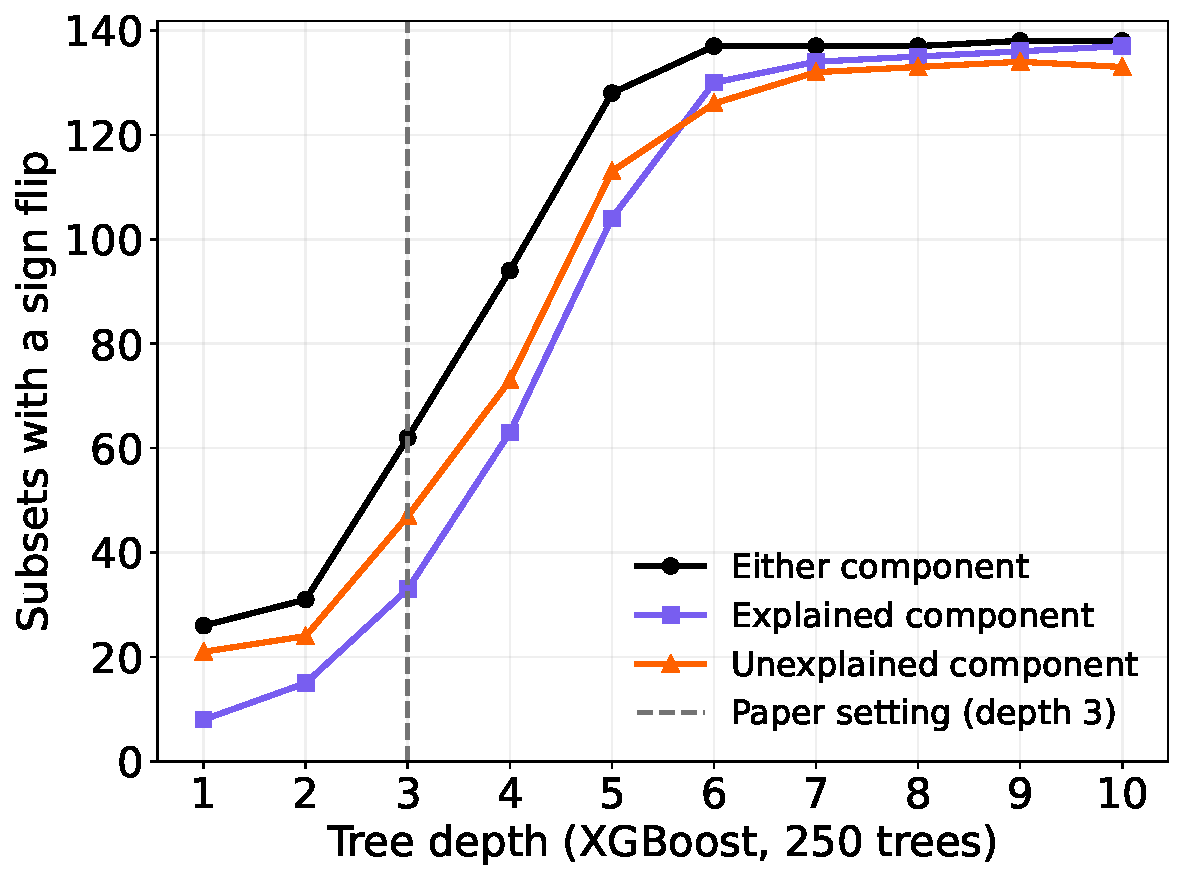
\includegraphics[width=0.3\textwidth]{Sections/Figures/complexity/icu_xgb_depth.pdf}} &
    \raisebox{-0.5\height}{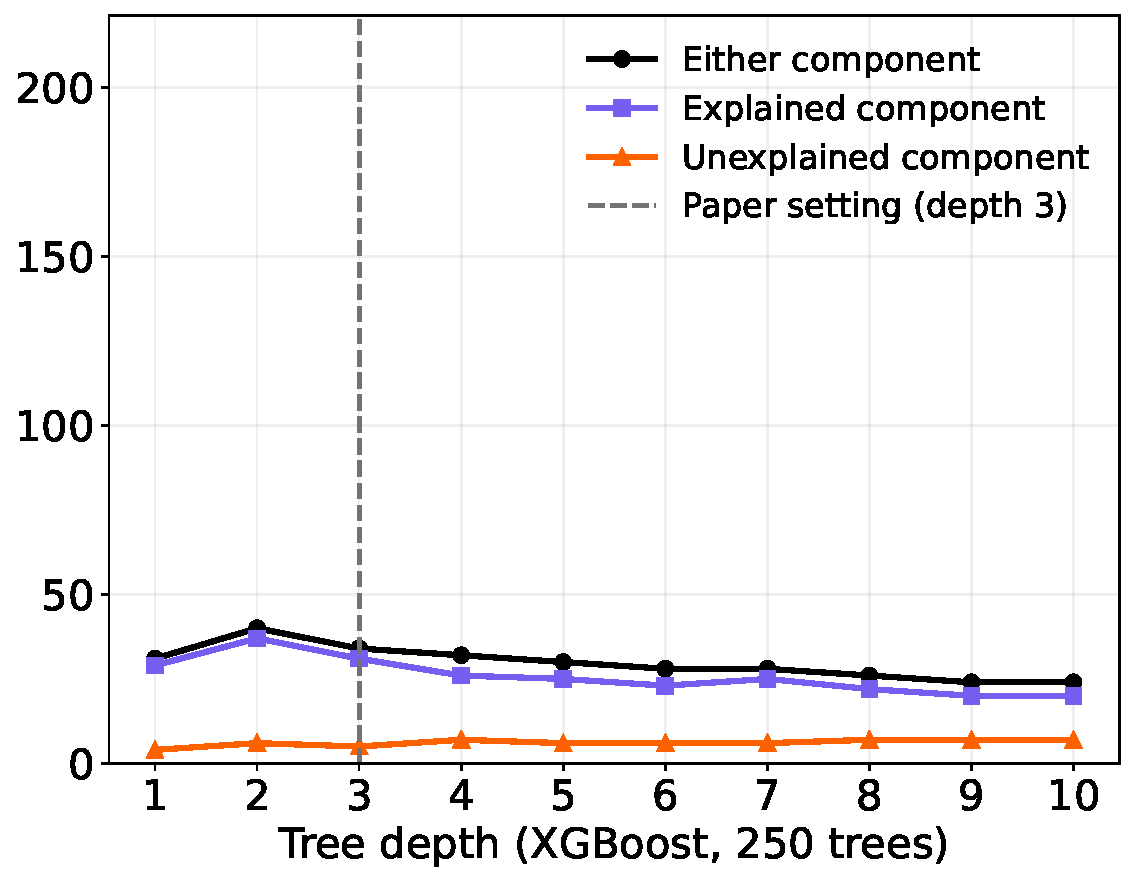
\includegraphics[width=0.3\textwidth]{Sections/Figures/complexity/census_xgb_depth_pincp_noylabel.pdf}} &
    \raisebox{-0.5\height}{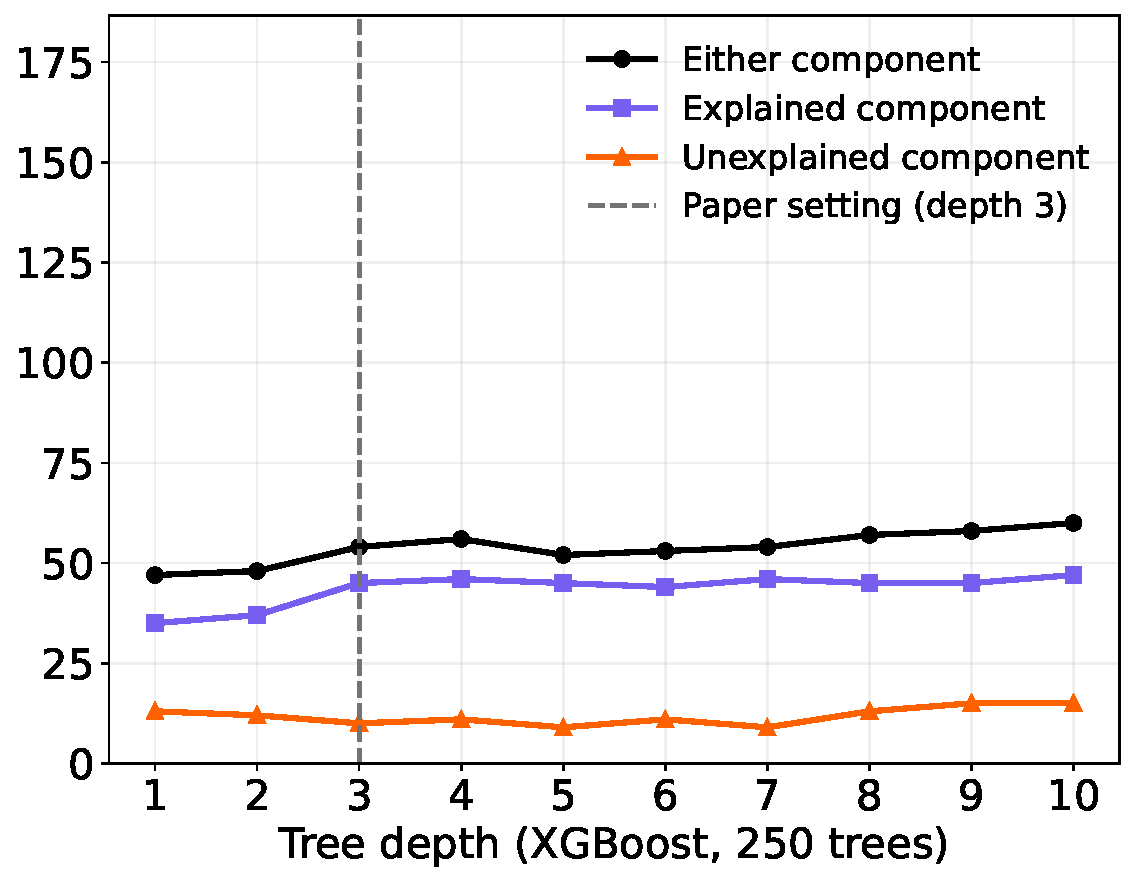
\includegraphics[width=0.3\textwidth]{Sections/Figures/complexity/census_xgb_depth_hicov_noylabel.pdf}} \\[2pt]
    \rotatebox[origin=c]{90}{\small XGBoost: number of trees} &
    \raisebox{-0.5\height}{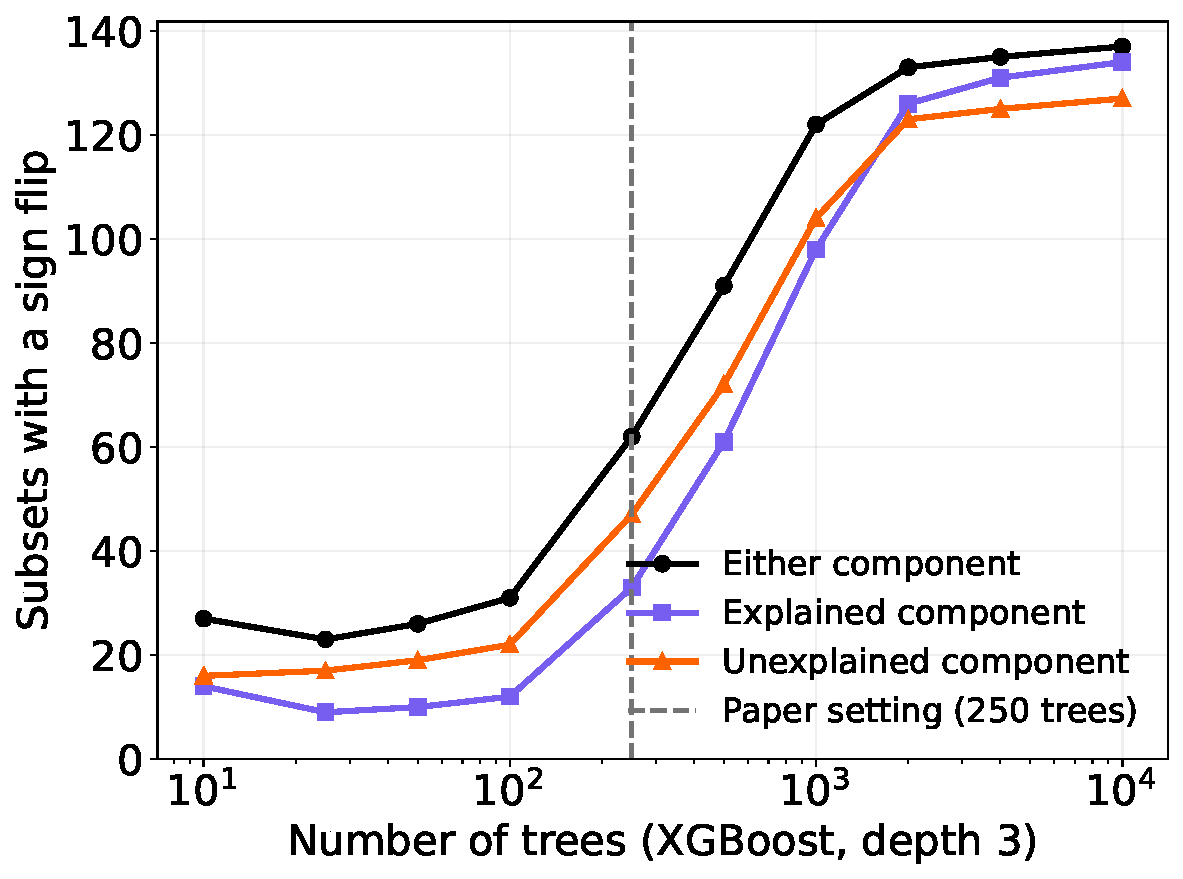
\includegraphics[width=0.3\textwidth]{Sections/Figures/complexity/icu_xgb_trees.pdf}} &
    \raisebox{-0.5\height}{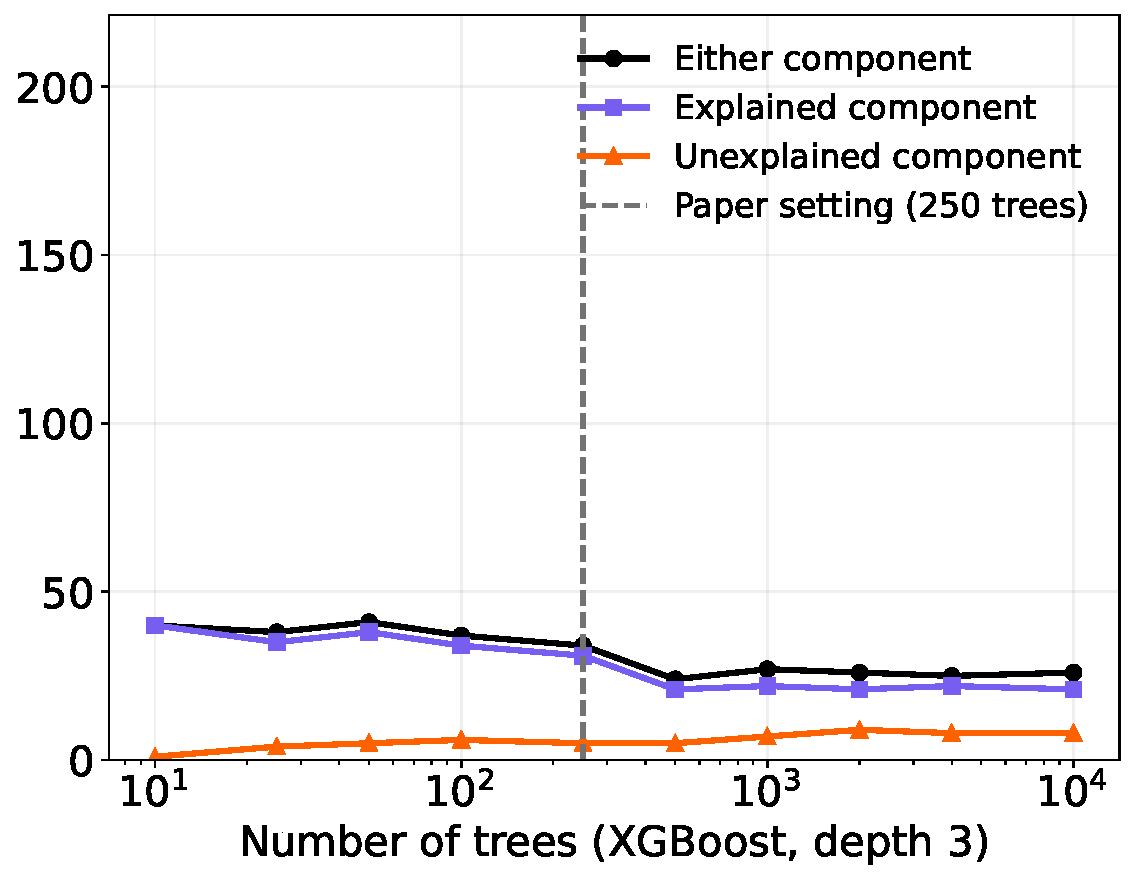
\includegraphics[width=0.3\textwidth]{Sections/Figures/complexity/census_xgb_trees_pincp_noylabel.pdf}} &
    \raisebox{-0.5\height}{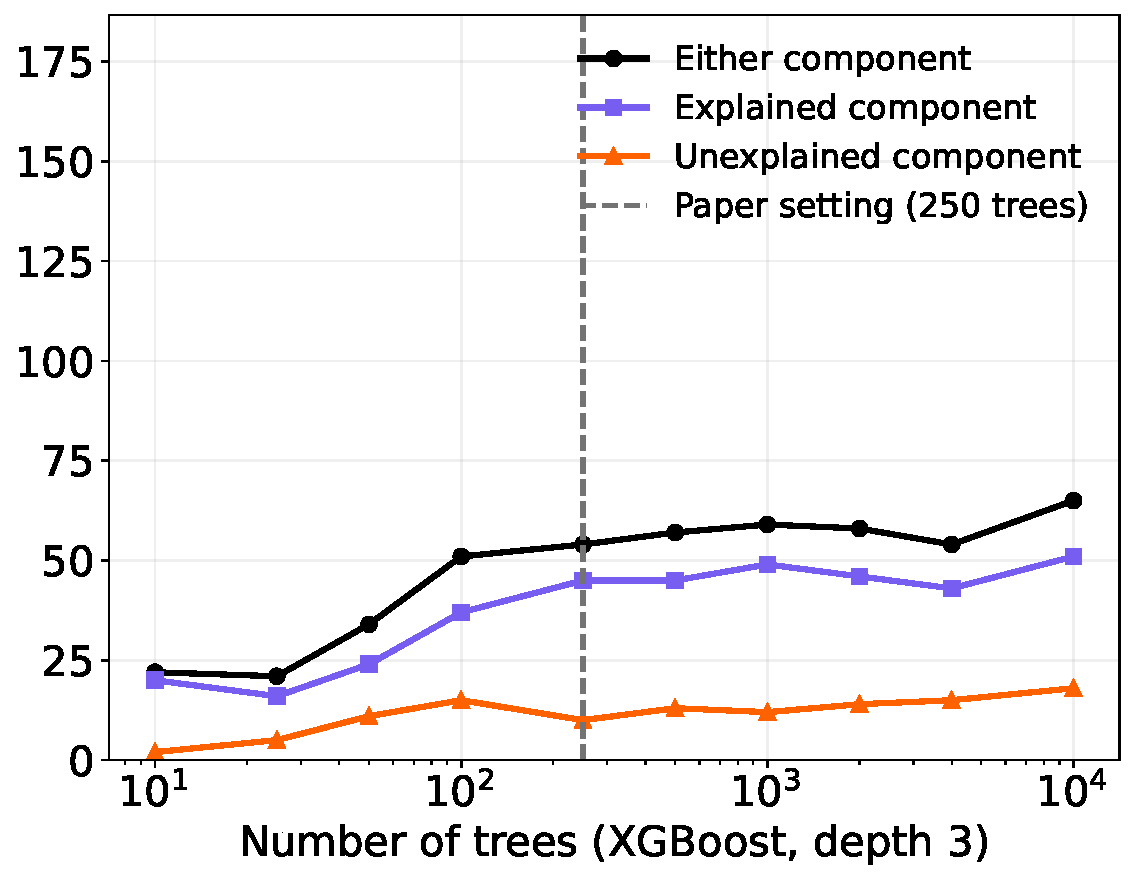
\includegraphics[width=0.3\textwidth]{Sections/Figures/complexity/census_xgb_trees_hicov_noylabel.pdf}} \\[2pt]
    \rotatebox[origin=c]{90}{\small Neural network: width} &
    \raisebox{-0.5\height}{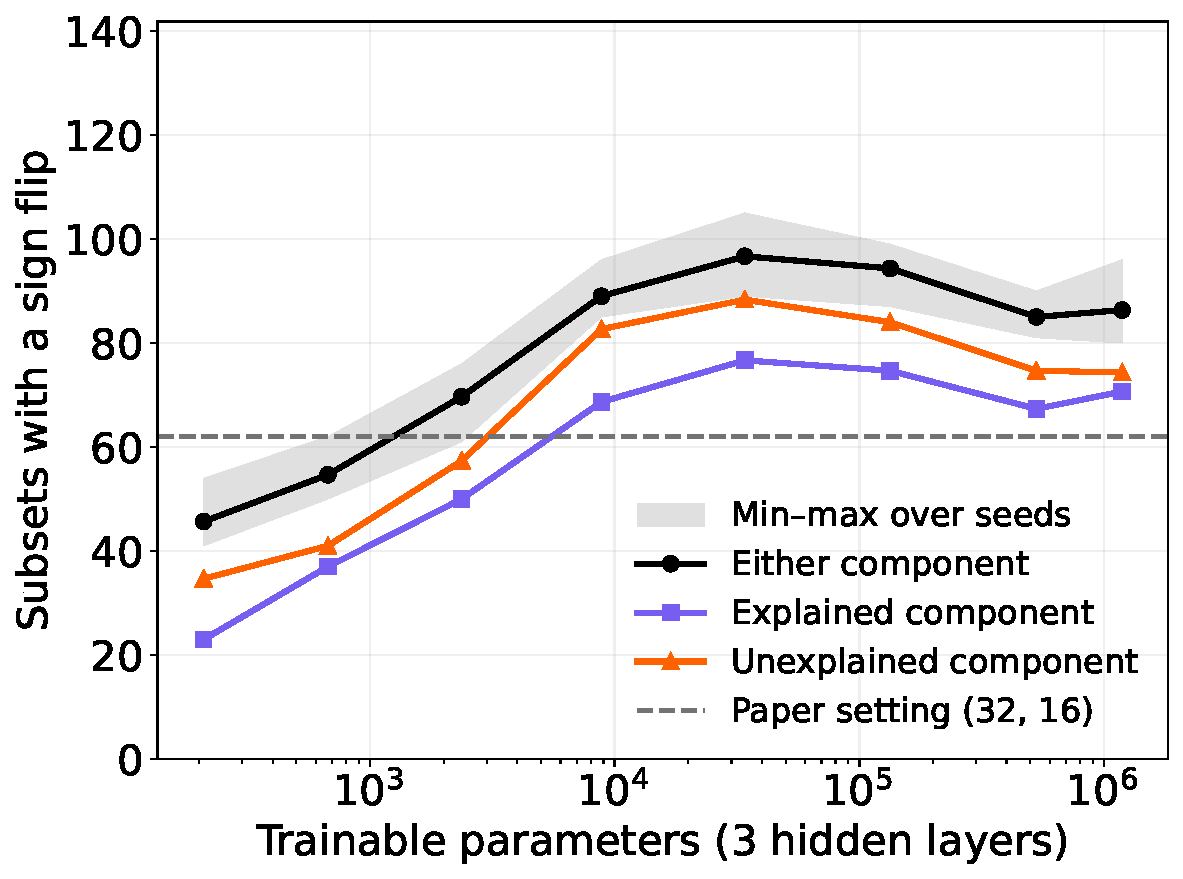
\includegraphics[width=0.3\textwidth]{Sections/Figures/complexity/icu_nn_width.pdf}} &
    \raisebox{-0.5\height}{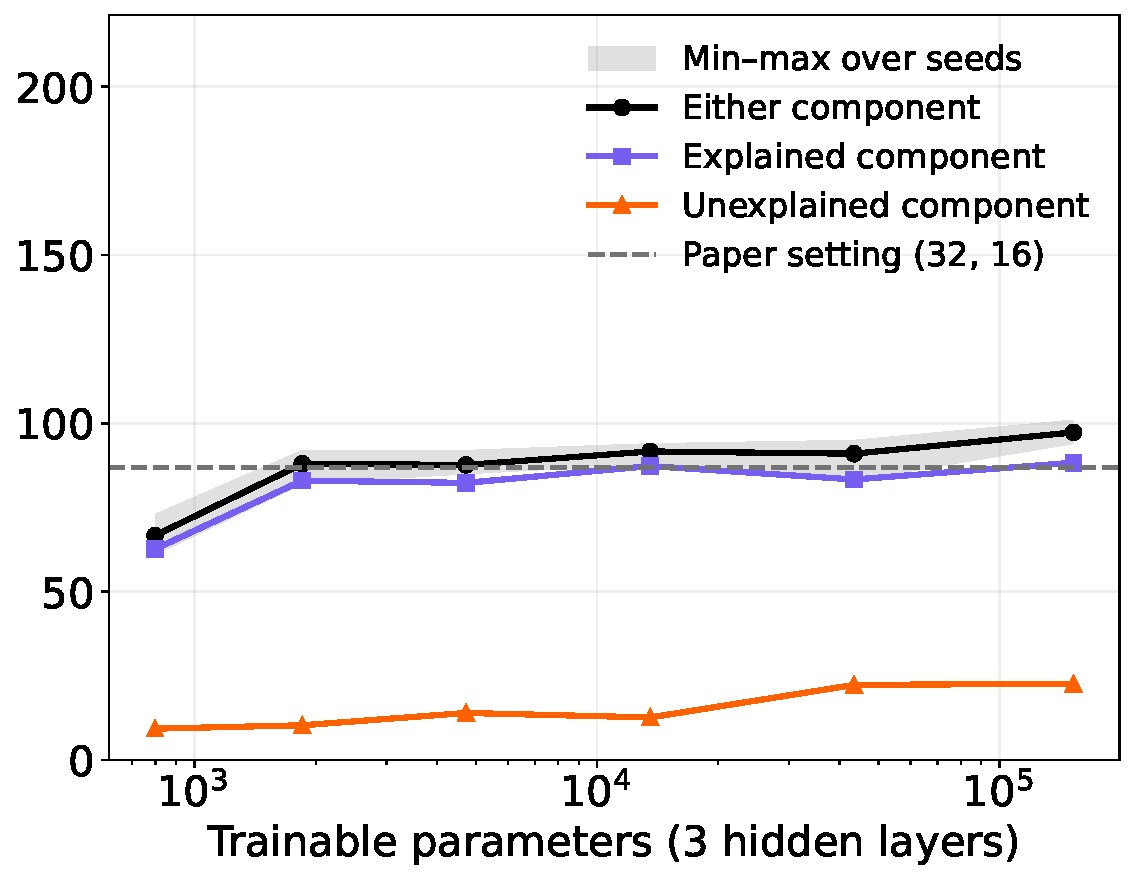
\includegraphics[width=0.3\textwidth]{Sections/Figures/complexity/census_nn_width_pincp_noylabel.pdf}} &
    \raisebox{-0.5\height}{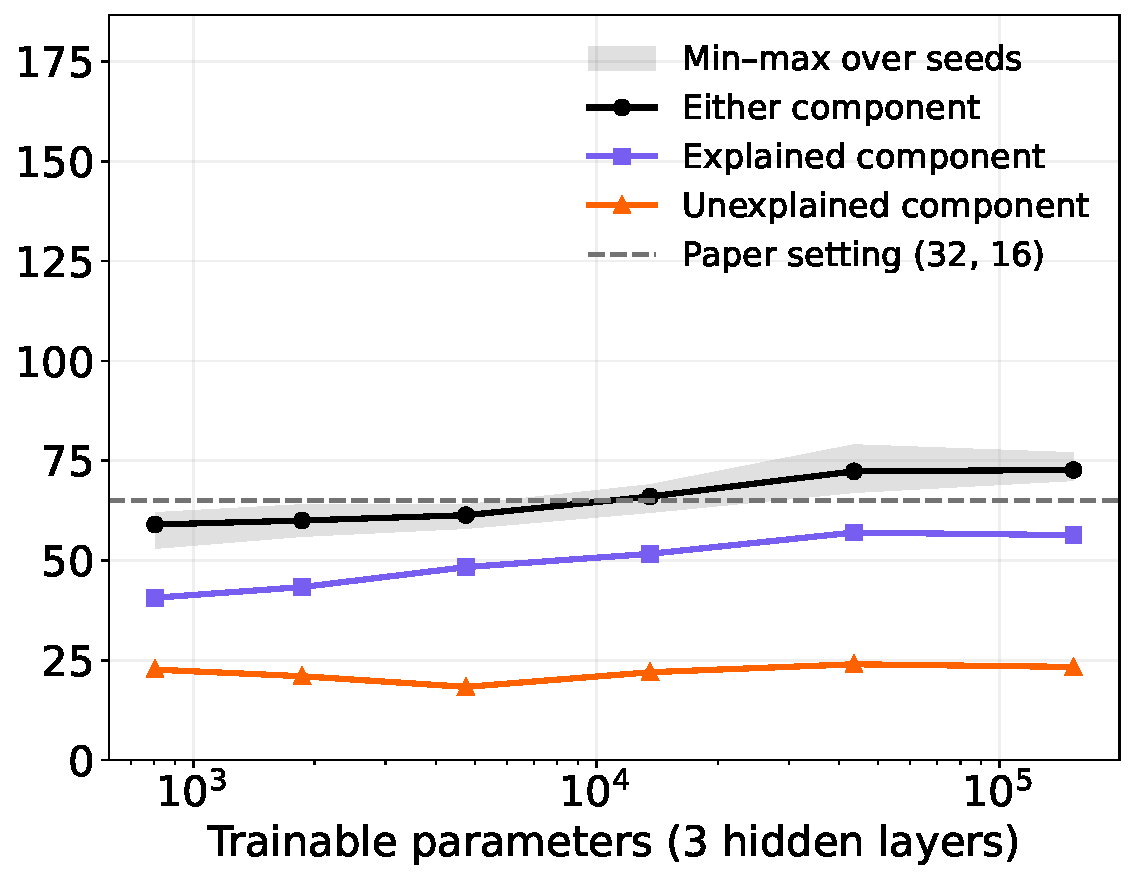
\includegraphics[width=0.3\textwidth]{Sections/Figures/complexity/census_nn_width_hicov_noylabel.pdf}} \\[2pt]
    \rotatebox[origin=c]{90}{\small Neural network: depth} &
    \raisebox{-0.5\height}{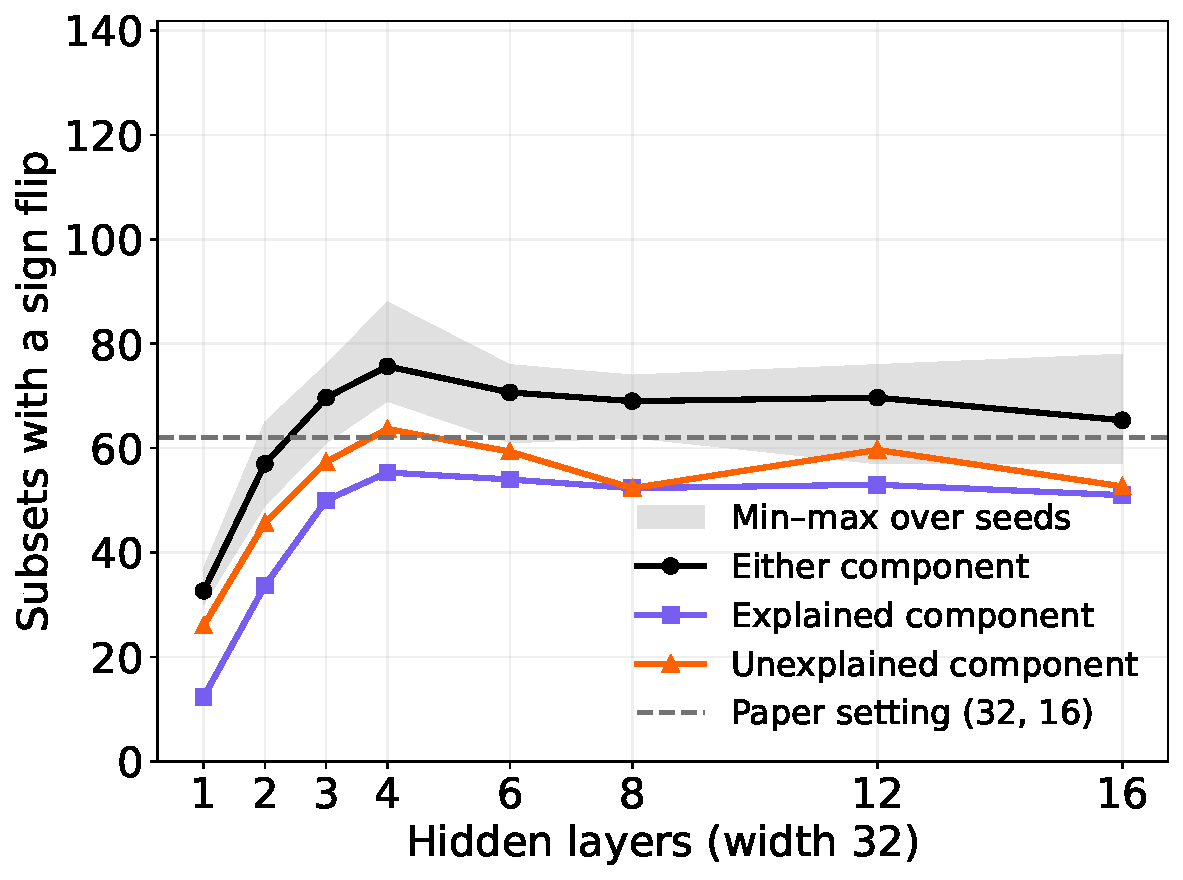
\includegraphics[width=0.3\textwidth]{Sections/Figures/complexity/icu_nn_depth.pdf}} &
    \raisebox{-0.5\height}{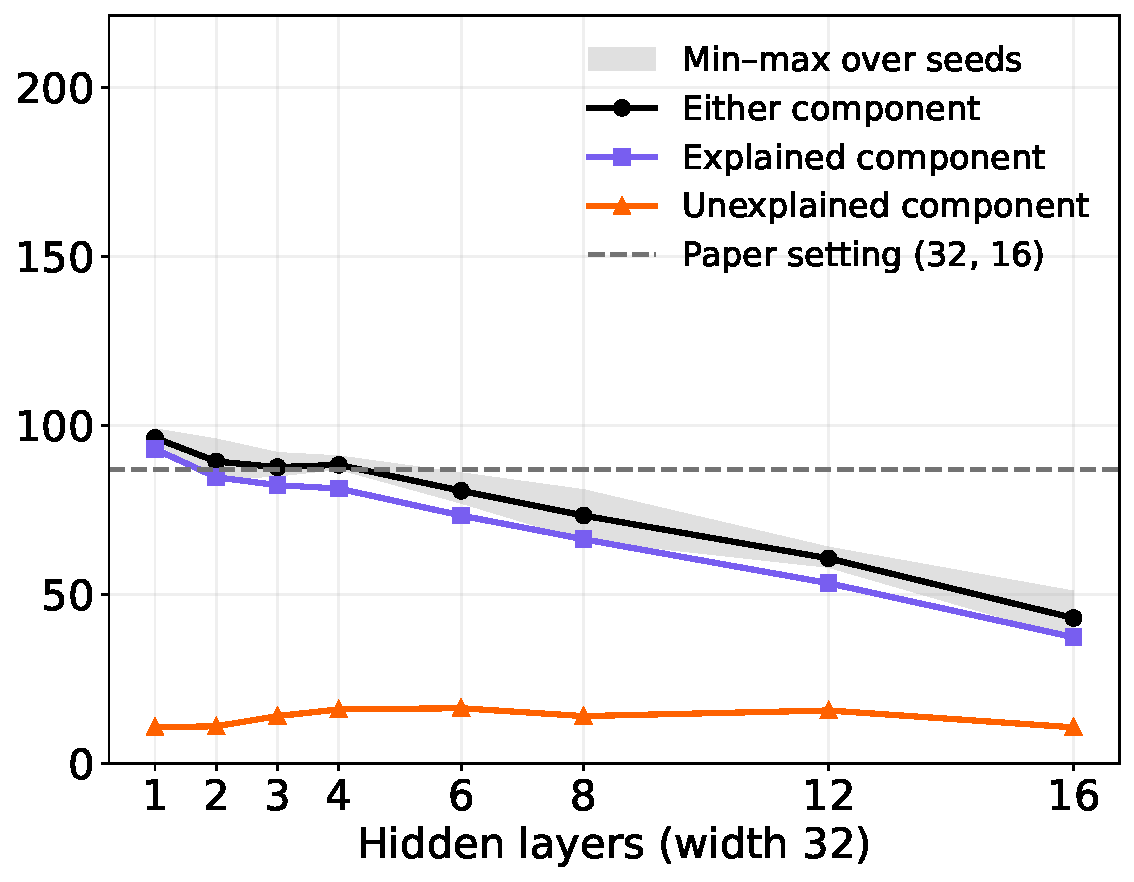
\includegraphics[width=0.3\textwidth]{Sections/Figures/complexity/census_nn_depth_pincp_noylabel.pdf}} &
    \raisebox{-0.5\height}{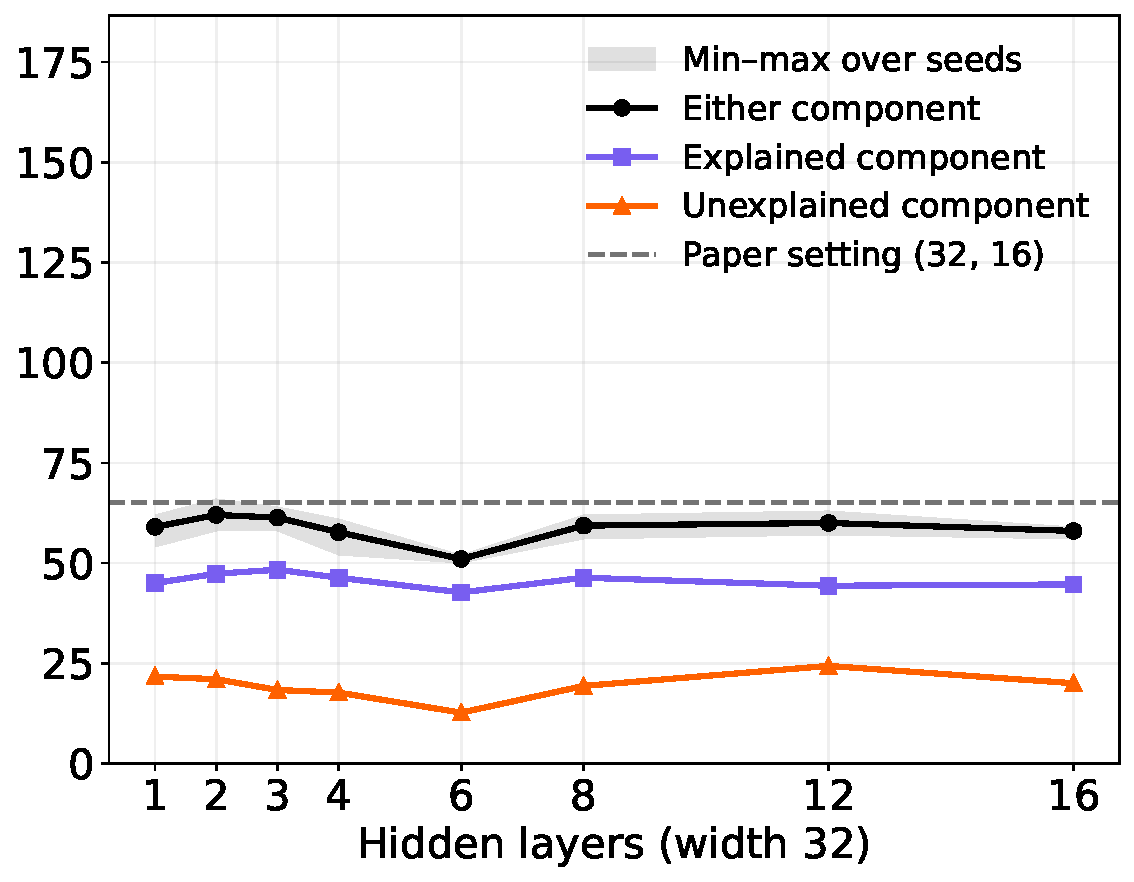
\includegraphics[width=0.3\textwidth]{Sections/Figures/complexity/census_nn_depth_hicov_noylabel.pdf}} \\[2pt]
    \end{tabular}
    \caption{Number of data subsets with a sign flip as a function of model complexity, for the ICU data (left), Census log income (center), and Census health insurance (right). Rows vary the XGBoost tree depth, the XGBoost number of trees, the neural network width (three hidden layers of equal width; horizontal axis is the number of trainable parameters), and the neural network depth (hidden layers of width $32$). Black: either component; purple: explained component; orange: unexplained component. The dashed line marks the setting reported in \cref{tab:flip_summary_main,tab:flips_census_income,tab:flips_census_insurance}. For the neural network, lines are means over three initialization seeds and the shaded band is the range across seeds.}
    \label{fig:complexity_sweeps}
    }
\end{figure*}
